\chapter{Event reconstruction and simulation}
\label{chap:reconstruction}

After the result of proton collisions have been observed in the
various subdetectors that comprise \CMS, each of these events must be
reconstructed in a way that allows for analysis of the physical
processes occurring in the collision. Information from the
subdetectors is used to infer the presence of different particles
produced in the collision. To help understand the different physical
processes that may occur during \LHC proton collisions \MC simulations
of events are utilised. The reconstruction algorithms and simulations
that are relevant to a search for supersymmetry are described in this
Chapter.

\section{Tracks and vertices}
\label{sec:tracks_reco}

As charged particles pass through the \CMS tracker they leave energy
deposits, known as ``hits'', in each layer. These
hits are reconstructed as tracks with the \ac{CTF}
algorithm \cite{Chatrchyan:2014fea}. This algorithm tries to associate
hits that belong to a single charged particle. This allows the
determination of the track left by the charged particle its curvature
through the magnetic field can be measured. The steps of the algorithm
are as follows:

\begin{itemize}
\item{Initially two or three hits in the inner layers of the tracker
are used to produce seeds for initial track candidates. Quality
selections are applied on the selected hits to reduce the number of fake tracks.} 
\item{Each seed is extrapolated along the expected trajectory using a
Kalman filter \cite{Fruhwirth:1987fm} with a helical tracking
hypothesis.  This allows the seeds to be associated with hits in an
outer tracker layer.} 
\item{The extrapolation is carried out recursively into the subsequent
tracker layers until the outer-most layer, or another
stopping condition, is reached.} 
\item{Of the tracking candidates that are found, additional quality
criteria are required to reject fake tracks.}
\item{This series of steps is repeated up to six times with the hits
associated to identified tracks removed after each iteration. }
\end{itemize}

Track reconstruction efficiencies for a variety of charged particles
are shown in Fig.~\ref{fig:tracks_reco} as a function of \pt and
$\eta$. In the central region of the detector all particles with a \pt
from 10 to 100~\gev are reconstructed with a 90-100\% precision. In the
forward detector region this efficiency remains above $\sim80\%$.
%fake rate? leave out for now...

\begin{figure}
\begin{center}
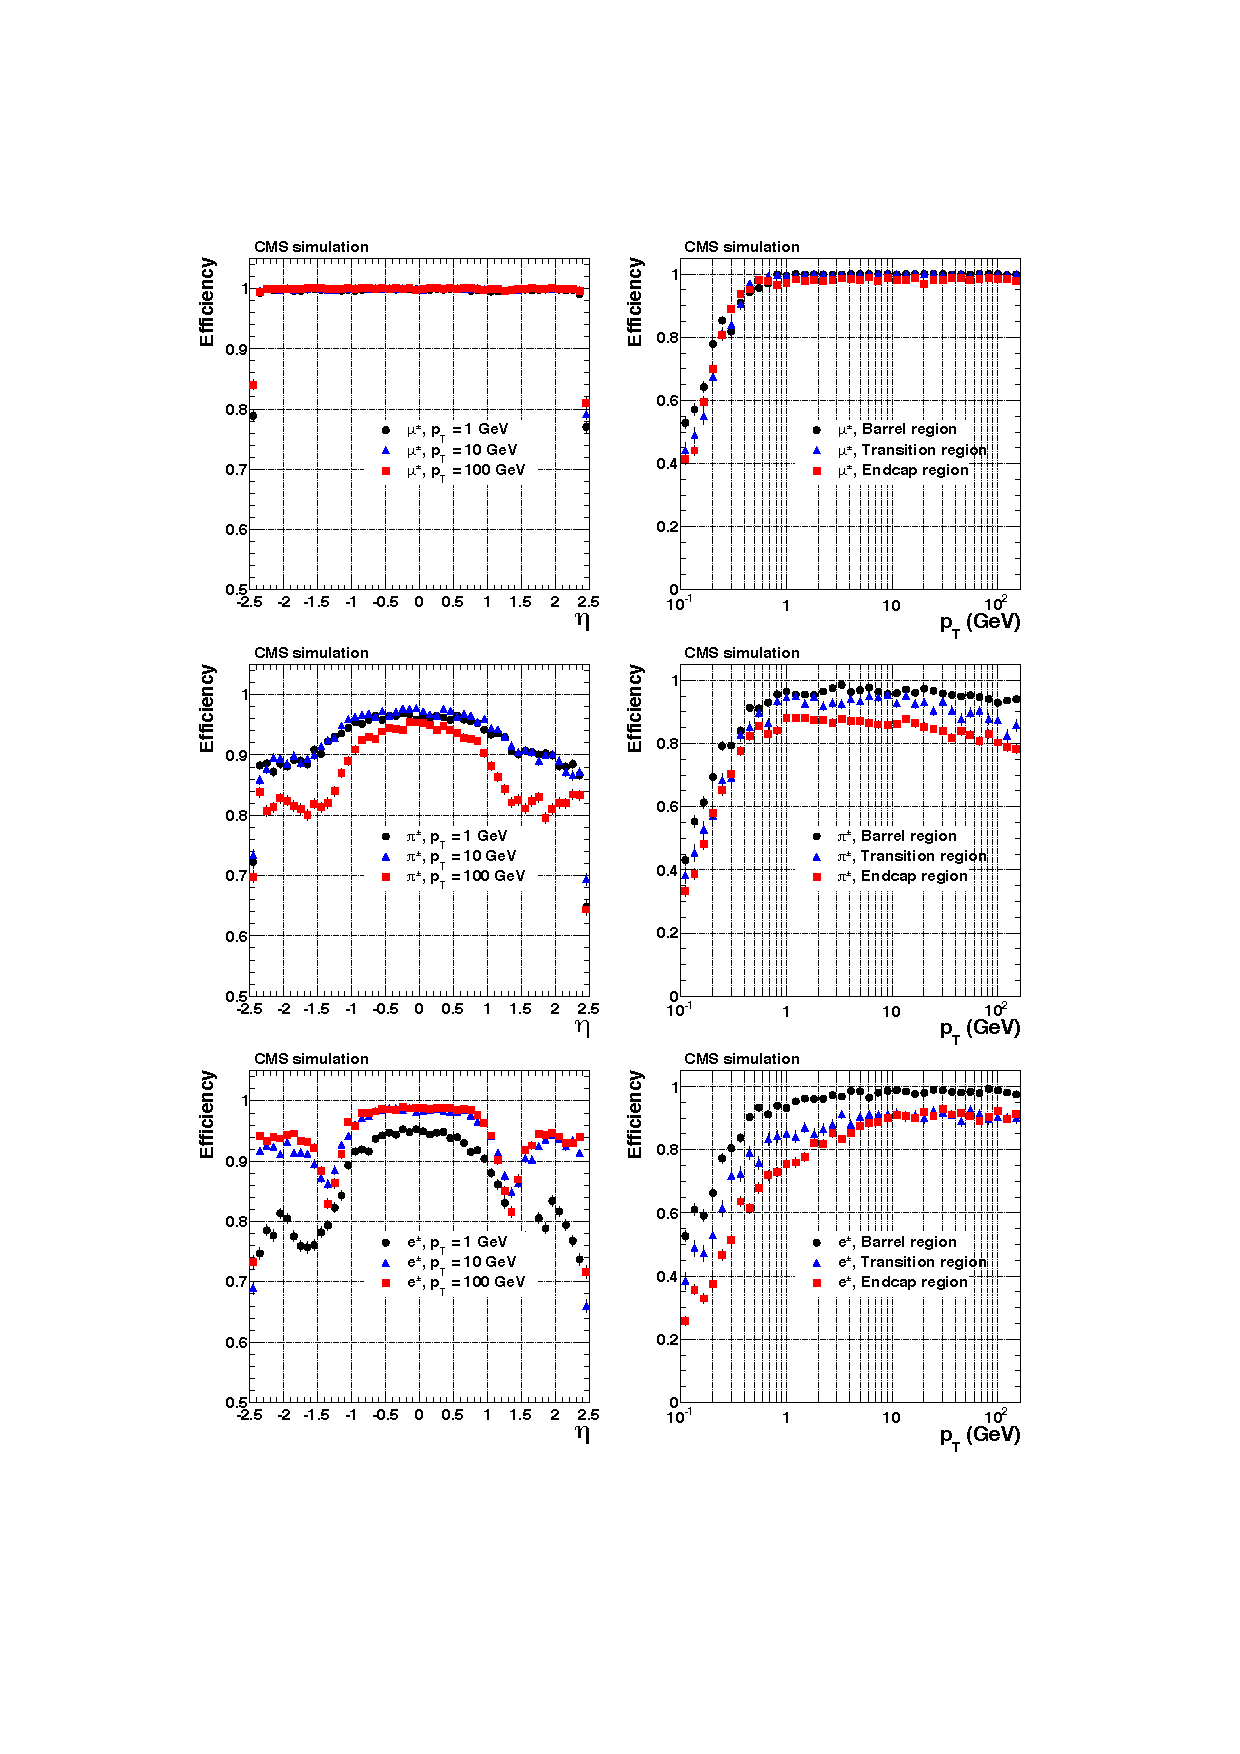
\includegraphics[width=0.8\linewidth]{figs/reconstruction/trackerPerformance} \end{center}
\caption{Efficiencies of track reconstruction for different charged
particles as a function of \pt and $\eta$. Muons are shown at the top,
pions in the middle and electrons at the bottom. The barrel,
transition and endcap regions are defined by the $\eta$ intervals of
0-0.9, 0.9-1.4 and 1.4-2.5 respectively.  For all the tracks
``high-purity'' quality requirements are made
\cite{Chatrchyan:2014fea}}
\label{fig:tracks_reco} \end{figure}

After charged particle tracks are reconstructed they can be used to
reconstruct the positions, known as interaction vertices, of the different
proton-proton in the event. Tracks are required to originate from a
region that is compatible with the \LHC ``beamspot'', the area in
which the proton beams cross and collisions occur. The $z$ coordinates
of tracks at the closest point of approach to the beamspot are taken
as an input for the deterministic annealing clustering algorithm
\cite{726788:DA}. This finds the most probable vertex positions and
assigns each track to a vertex. The final $x$,$y$,$z$ position of
these vertices is then found using the adaptive vertex fitter 
\cite{Waltenberger:2008zz}. This assigns the most probably position of
the vertex for the given set of input tracks. Quality criteria are
then applied to reject fake vertices. They are chosen in such a way as
to remain efficient for real vertices that typically have a large
number of tracks compatible with them. Finally, the ``primary vertex''
is determined as the vertex with tracks that have the greatest scalar
sum of \pt. Other vertices are then initially attributed to \PU.
However, vertices that are displaced from the initial proton collision
are common signatures of unstable particles that decay within the
detector, such as $b$-hadrons. These can be found in subsequent levels
of reconstruction.

The primary vertex efficiency as a function of the number of tracks in
a cluster can be seen in Fig.~\ref{fig:vertex_reco}. The efficiency increases to
close to $>99\%$ as long as there are a reasonable number of tracks in
an event. The vertex resolution reaches $\sim10~\mu$m in $x,y$ and
$\sim10~\mu$m in $z$ with $>40$ reconstructed tracks.

\begin{figure}
\begin{center}
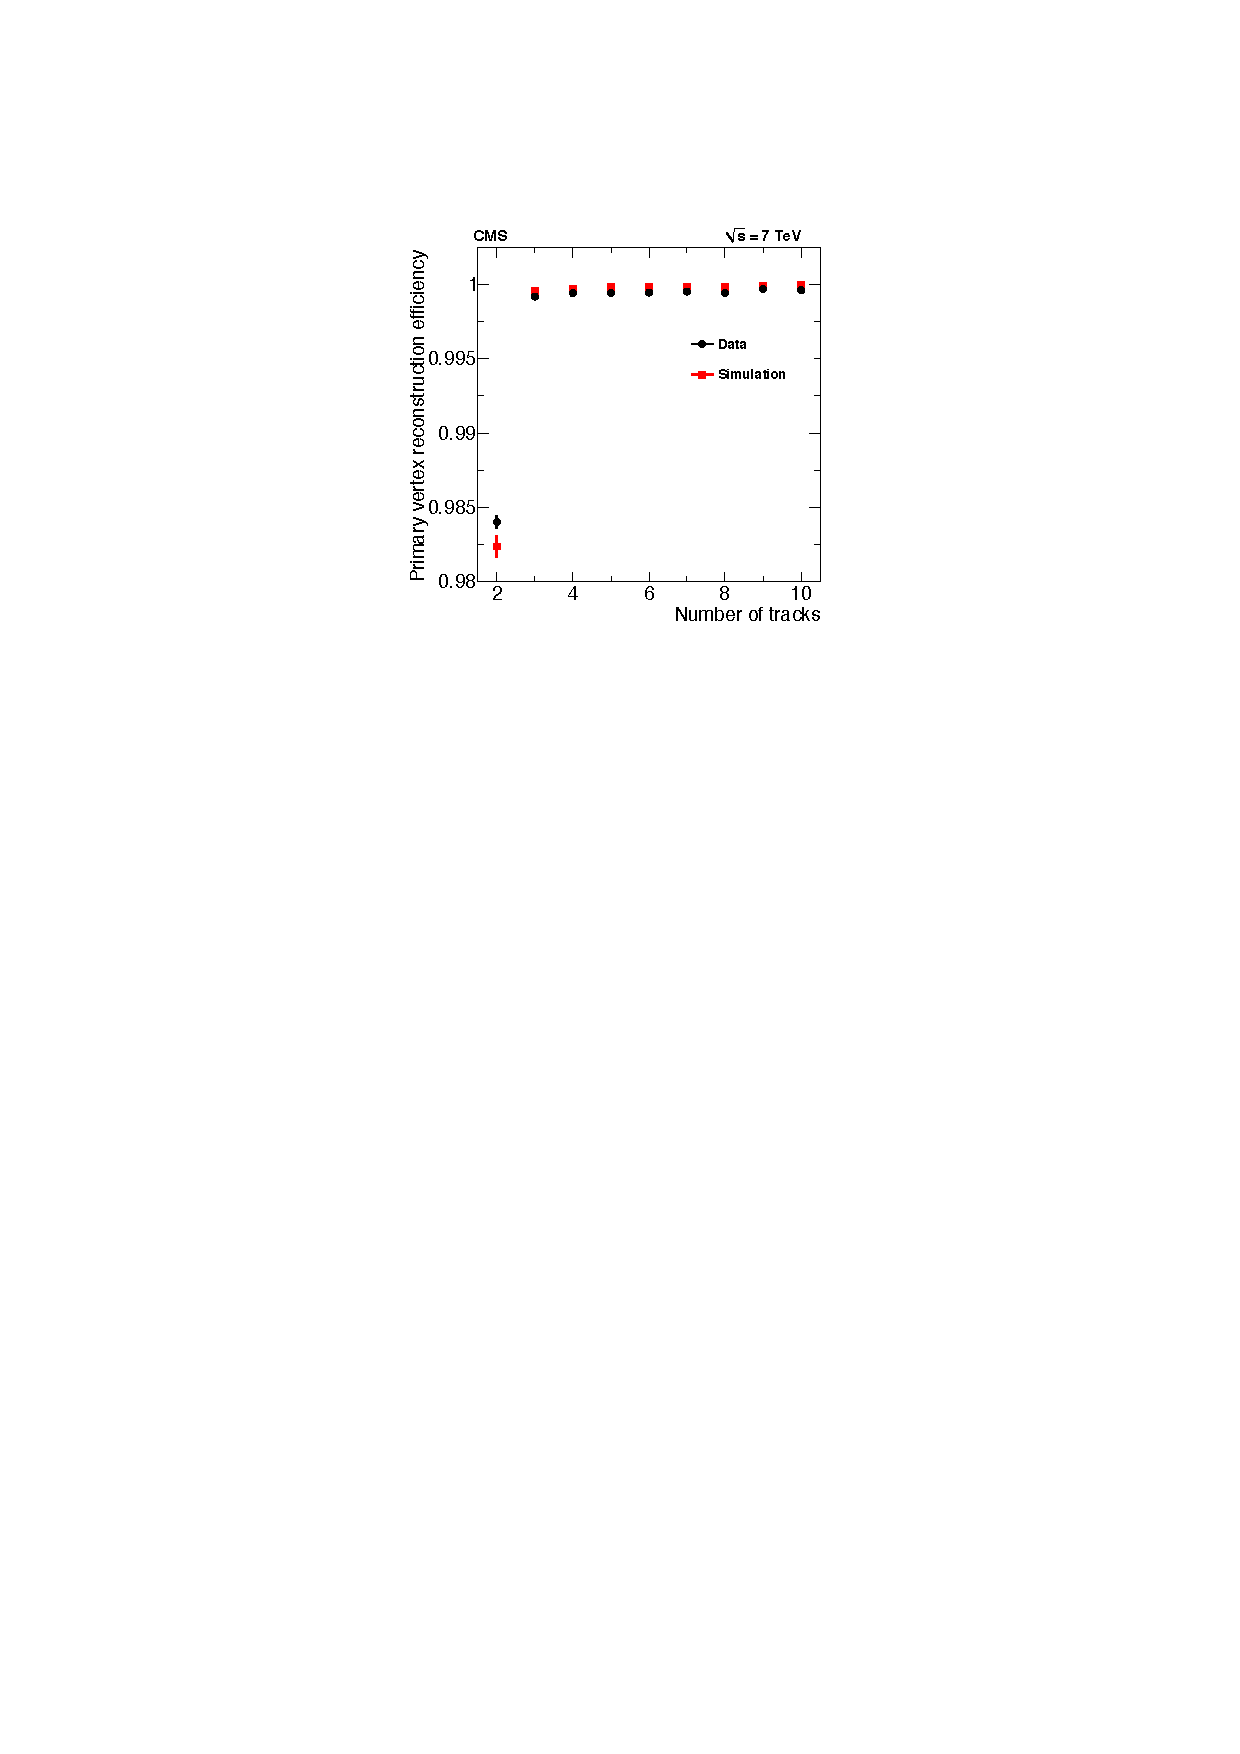
\includegraphics[width=0.5\linewidth]{figs/reconstruction/vertexPerformance} \end{center}
\caption{ The vertex reconstruction efficiency as a function of the
number of tracks originating from the vertex. Measured in data and
simulation for $\sqrt{s}=7~\tev$ proton collisions.
\cite{Chatrchyan:2014fea}}
\label{fig:vertex_reco} \end{figure}


\section{Particle flow}
\label{sec:pflow_reco}

Each subdetector of \CMS contributes complimentary information about
the different types of particles that pass through the detector. This
complementary is exploited in identifying the different types of
particle with the \PF algorithm
\cite{CMS-PAS-PFT-09-001,CMS-PAS-PFT-10-001,CMS-PAS-PFT-10-002}. As
\CMS has accurate momentum resolution in the tracker and a high
granularity \ECAL this algorithm allows both to augment the
measurement of objects in the \HCAL. This then allows calibrations
specific to charged and neutral hadrons to be applied. 

The \PF algorithm searches for a set of individual particles that are
known as ``\PF candidates''. They are then classified as charged or
neutral hadrons, photons, muons or electrons. The set of \PF
candidates can then be utilised to calculate other event level
variables, such as for jet reconstruction described in
Sec.~\ref{sec:jets_reco}.
%Do i need to describe how clusters are made more?

The algorithm starts by taking the tracks, that are reconstructed as
described in Sec.~\ref{sec:tracks_reco}, along with clusters of energy
in the calorimeters, which are reconstructed separately in the \ECAL and
\HCAL. Clusters are paired with tracks if the track trajectory is
compatible with the cluster position. These pairs are then used to
identify charged particles. Electrons and hadrons are typically
differentiated based on the proportion of energy they deposit in the
\ECAL or \HCAL. Electrons will deposit nearly all their energy in the
\ECAL where hadrons will deposit much more in the \HCAL. A similar
pairing between tracks and hits in the muon system is used to identify
muons. 

Neutral particles are then identified through calorimeter clusters
that do not have a compatible track associated to them. Photons, for
example, will leave a significant \ECAL deposit with no track, which
would be present for electrons. Similarly, neutral hadrons will leave
significant deposits in the \HCAL with no associated track.

\section{Electrons and photons}
\label{sec:electrons_reco}

Both electrons and photons interact with the \ECAL in a similar way.
The reconstruction techniques used are therefore very similar, with
the main difference being the lack of track in photon reconstruction.
As electrons interact with the tracker, they lose $33\%$ of their
energy on average before reaching the \ECAL
\cite{1748-0221-10-06-P06005}. Most of this energy loss occurs through
bremsstrahlung, which is non-Gaussian. As the Kalman filter that is
used in track reconstruction assumes Gaussian energy losses another
specialist track reconstruction for electrons is employed, known as
the Gaussian Sum Filter algorithm \cite{Adam:815410}. The photons that
are produced during bremsstrahlung must also be properly associated to
the electron when clustering in the calorimeter to maintain a good
energy resolution. As the electrons bend in the magnetic field but
the photons they emit do not, the calorimeter clusters are allowed to
extend along the azimuthal direction. These rectangular \ECAL windows
are know as ``superclusters''.

super cluster reconstruction 

hybrid in barrel , multi 5x5 in the endcap

\section{Muons}
\label{sec:muons_reco}

don't lose much energy


\section{Jets}
\label{sec:jets_reco}

\section{Missing transverse energy (MET)}
\label{sec:met_reco}

\section{Monte Carlo (MC) simulation}
\label{sec:mc_reco}

